\section{Processi primari}
\subsection{Fornitura}
Verranno ora trattate le norme che i membri di duckware devono rispettare per poter diventare fornitori nei confronti di \emph{Zero12} e dei committenti, \emph{Prof. Tullio Vardanega} e \emph{Prof. Riccardo Cardin}.
\subsubsection{Studio di fattibilità}
In data \emph{16 Novembre 2018} è avvenuta presso la Torre Archimede la presentazione dei capitolati d’appalto da parte di alcune aziende interessate nel coinvolgimento degli studenti in un progetto. Il giorno \emph{20 Novembre 2018} è stata organizzata una riunione del gruppo per discutere di vari argomenti, primo fra tutti la scelta dei capitolati più interessanti da analizzare.
Dopo aver scelto il capitolato per il quale proporsi è stata eseguita un’ulteriore analisi relativa ai rischi ed alle opportunità che è stata riportata all’interno dello \emph{Studio di fattibilità 1.0.0}. Si tratta di un documento nel quale viene indicato, per ogni capitolato, le motivazioni per le quali il gruppo \textbf{duckware} vorrebbe proporsi come fornitore. In particolare, sono presenti per ogni capitolato:
\begin{itemize}
	\item Una descrizione del prodotto proposto dall’azienda secondo le regole del capitolato \emph{d’appalto};
	\item Una descrizione di quello che sarà l’ambito d’uso del prodotto che ci si propone di creare;
	\item Le tecnologie richieste dal capitolato per la realizzazione del relativo progetto;
	\item Le motivazioni fornite dal team \emph{duckware} riguardo l’accettazione o la respinta del capitolato in questione.
\end{itemize}
\subsection{Sviluppo}
\subsubsection{Analisi dei Requisiti}
L’analisi dei requisiti ha lo scopo di individuare i \markg{requisiti} richiesti dal capitolato preso in questione. Tali informazioni possono essere reperite da verbali, casi d’uso oppure dai capitolati d’appalto stessi. Il risultato finale di questa analisi porterà alla creazione da parte degli analisti del documento \emph{Analisi dei requisiti 1.0.0} che fornirà informazioni riguardo:
\begin{itemize}
	\item Descrivere l’obiettivo del lavoro del gruppo e fornire riferimenti precisi ai progettisti;
	\item Fornire una lista dettagliata di funzionalità e \markg{requisiti} concordati col  cliente;
	\item Fornire degli esempi di dialoghi tra l'utente e l'assistente vocale, riferiti alle funzionalità che necessitano di un iterazione tra i due;
	\item Dare ai verificatori riferimenti e casi d’uso per poter creare ed eseguire dei test mirati ed affidabili;
	\item Rendere più semplice il \markg{processo} di revisione del codice.
\end{itemize}
\subsubsection{Classificazione di \markg{requisiti}}
Ogni \markg{requisito} è identificato da un codice che verrà rappresentato secondo quanto segue:
\begin{center}
	R.{x}.{y}.{z}
\end{center}
\begin{itemize}
	\item \textbf{R}: sta per Requisito;
	\item \textbf{X}: indica l’importanza di tale \markg{requisito} che può essere 0 (opzionale), 1 (\markg{requisito} non necessario ma può dare maggiore completezza e definizione) e 2 (obbligatorio in quanto necessario per il funzionamento basilare);
	\item \textbf{Y}: assume valore F se \markg{requisito} funzionale, Q se di qualità, V se di vincolo e P se presentazionale.
\end{itemize}
Gli analisti avranno anche cura di identificare i casi d’uso i quali verranno descritti secondo il seguente schema:
\begin{center}
	\textbf{UC[Codice principale].[Codice secondario].[Codice terziario][Codice quaternario] – Identificativo}
\end{center}
\begin{itemize}
	\item \textbf{UC} e \textbf{Identificativo}: Ogni caso d’uso è specificato da una serie di cifre spaziate da un punto. La prima cifra indica il numero del padre, la seconda invece il numero del figlio. Un trattino separera il tutto dal nome univoco del caso d’uso;
	\item \textbf{Attori}: gli attori principali e secondari dell’UC (use case);
	\item \textbf{Scopo} e \textbf{descrizione}: una descrizione riassuntiva del caso d’uso;
	\item \textbf{Scenario principale}: usando una lista numerata indica il flusso degli eventi specificando per ognuno a quale caso d’uso si riferisce;
	\item \textbf{Voice flow}: descrive l'eventuale iterazione vocale tra l'utente e l'assistente \markg{Alexa};
	\item \textbf{Estensioni}: contiene una lista degli eventuali errori che il \markg{caso d'uso} può generare;
	\item \textbf{Pre-condizione}: specifica le condizioni vere prima del verificarsi degli eventi del caso d’uso;
	\item \textbf{Post-condizione}: specifica le condizioni vere dopo il verificarsi degli eventi del caso d’uso.
\end{itemize}
\subsection{Progettazione}
\subsubsection{Scopo}
La progettazione ha il compito di disegnare, attraverso i Progettisti, una soluzione del problema che sia esaustiva per tutti gli \markg{stakeholders}. Verrà definita la logica del prodotto identificando i componenti e cercando sempre di restare nei costi che sono stati prefissati. In particolare la logica definita dovrà:
\begin{itemize}
	\item Soddisfare i \markg{requisiti} dell’\emph{Analisi dei requisiti} ed adattarsi ai cambiamenti od alle evoluzioni che potenzialmente avverranno nel tempo;
	\item Essere comprensibile e modulare;
	\item Avere la capacità di rispettare le specifiche nel tempo, anche nel caso di malfunzionamenti;
	\item Ridurre al minimo i tempi di manutenzione.
\end{itemize}
\subsubsection{Diagrammi}
Le scelte adottate dai progettisti verranno adeguatamente descritte attraverso l’uso di diagrammi \markg{UML} 2.0 per rendere più chiare e meno ambigue le decisioni prese. Verranno in particolare utilizzare le seguenti rappresentazioni:
\begin{itemize}
	\item \textbf{Diagrammi di casi d’uso}: descrivono le funzioni del sistema;
	\item \textbf{Diagrammi delle classi}: descrivono gli oggetti e le dipendenze fra essi;
	\item \textbf{Diagrammi dei \markg{package}}: descrivono la dipendenza tra i \markg{package} (i quali contengono le classi);
	\item \textbf{Diagrammi di sequenza}: descrivono la collaborazione nel tempo degli oggetti;
	\item \textbf{Diagrammi di attività}: descrivono la logica procedurale.
\end{itemize}
\subsubsection{Obiettivi della progettazione}
La progettazione garantisce che il prodotto finale soddisfi tutte le richieste emerse e specificate durante l’analisi. Deve garantire la qualità del prodotto sviluppato e cercare di ottimizzare l’uso delle risorse disponibili. Inoltre, una buona progettazione cerca di suddividere nel migliore dei modi i compiti implementativi al fine di ridurre la complessità del problema e, di conseguenza, facilitare il compito dei programmatori.
\subsection{Codifica}
I programmatori dovranno rispettare alcune regole che garantiranno uniformità e coesione al codice che verrà prodotto durante la creazione del progetto. Ci sono sia delle norme globali alle quali i programmatori si devono attenere, indipendentemente dal linguaggio di programmazione scelto, sia delle norme specifiche legate al linguaggio \markg{Java}.\\[0.5cm]
Per chiarezza ogni norma avrà un suo paragrafo composto di titolo, descrizione ed esempio illustrativo di quanto si vuole specificare.\\[0.5cm]
\textbf{Convenzioni per i nomi}
\begin{itemize}
	\item Ogni nome deve essere unico e soprattutto deve essere appropriato, ovvero deve descrivere al meglio ciò che rappresenta;
	\item In caso di nome formato dalla composizione di più parole, si potrà utilizzare l’underscore come separatore. In alternativa, si potranno separare i termini con una lettera maiuscola secondo la modalità detta \textit{lower\markg{CamelCase}}. Ad esempio:
	\begin{itemize}
		\item \texttt{variable\char`_name}
		\item \texttt{ANOTHER\char`_EXAMPLE\char`_FOR\char`_THIS}
		\item \texttt{yetAnotherExample}
	\end{itemize}
	\item Usare le lettere maiuscole quando si intende utilizzare una parola come attributo \emph{const} (costante). Altrimenti, usare lettere minuscole. Per esempio:
	\begin{itemize}
		\item \emph{(costante)} \texttt{variable\char`_name}
		\item (\textbf{non} costante) \texttt{ANOTHER\char`_EXAMPLE\char`_FOR\char`_THIS}
		\item (\textbf{non} costante) \texttt{yetAnotherExample}
	\end{itemize}
\end{itemize}
\textbf{Convenzioni per la documentazione}
\begin{itemize}
	\item I commenti ed i nomi presenti nel documento devono tassativamente essere scritti in inglese;
	\item Ogni file dovrà contenere nella sua intestazione, come commento, la seguente struttura:
\end{itemize}
\begin{figure} [h]
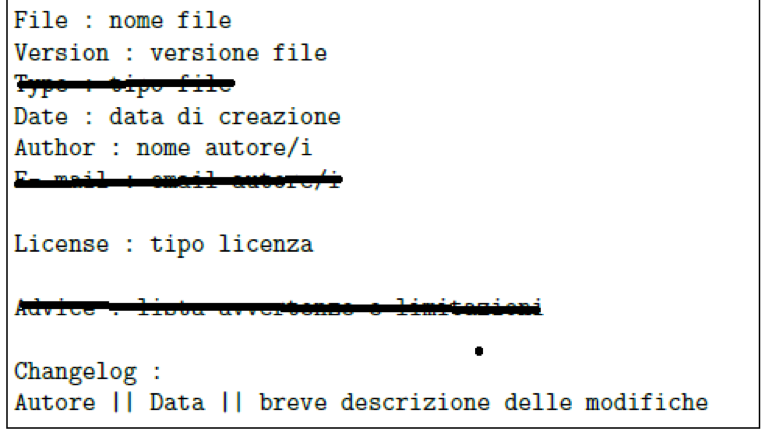
\includegraphics[width=1\textwidth]{../includes/pics/foto2_4.png}
\caption{Esempio convenzioni per la documentazione}
\end{figure}
\begin{itemize}
	\item La versione va inserita come X.Y dove:
	\begin{itemize}
		\item \textbf{X}: indica la versione principale ed è da incrementare \textbf{solo ed esclusivamente} nel caso in cui si passi ad una versione stabile. Un tale incremento comporta l’azzeramento di Y
		\item \textbf{Y}: indica la versione parziale ed un incremento di tale indice rappresenta una \markg{verifica} o una modifica rilevante che verrà sottoposta alla fase di test
	\end{itemize}
\end{itemize}
\subsubsection{\markg{Java}}
In questa sezione vengono indicate delle convenzioni adottate dal team di 
\href{https://google.github.io/styleguide/javaguide.html}\emph{Google} che dovranno essere rispettate nel progetto dagli sviluppatori durante la scrittura del codice.
\paragraph{Commenti}I commenti su singola riga possono essere inseriti tramite l’uso di un doppio slash \emph{(single line comment block)} oppure da uno slash seguito da un asterisco \emph{(multi-line comment block)}. Quest’ultima tecnica deve essere utilizzata anche per i commenti su più righe dove, per ciascun inizio di riga, deve essere presente un asterisco. È necessario inserire uno spazio dopo ogni asterisco di inizio riga, se presente.
\begin{table} [H]
	\begin{center}
		\begin{tabular}{ | l | l |}
			\multicolumn{1}{c}{\textbf{OK}}&\multicolumn{1}{c}{\textbf{NO}}\\ 
			\hline
			//commento su singola riga & //commento\\
			& //su più\\
			/* commento su singola riga */& //righe\\
			&\\
			/* commento&/*commento\\
			\hspace{0.2cm}* su più&\hspace{0.2cm}*su più\\
			\hspace{0.2cm}* righe */&\hspace{0.2cm}*righe*/\\
			\hline
		\end{tabular}
	\end{center}
	\caption{Esempio commenti}
\end{table}
Ogni file \texttt{.java} dovrà contenere in testa un commento a singola o multipla riga che descriva brevemente il contenuto del file e le funzionalità che offre.
\paragraph{Identazione}
Il corpo di ogni funzione dovrà essere separato dall’inizio della riga con una tabulazione, lasciando le impostazioni standard fornite dall’\markg{IDE}. In caso di istruzioni di controllo annidate, ognuna dovrà essere propriamente incolonnata e spaziata da tabulazioni rispetto all'inizio della riga.
\begin{table} [H]
	\begin{center}
		\begin{tabular}{ | l | l |}
			\multicolumn{1}{c}{\textbf{OK}}&\multicolumn{1}{c}{\textbf{NO}}\\ 
			\hline
			double test(int a) \{ & double test(int a) \{\\
			\hspace{0.5cm}if (a > 5) \{ 			   &  if (a > 5) \{\\
			\hspace{1cm}return a * 10;          & \hspace{0.5cm}return a * 10;\\
		    \hspace{0.5cm}\} else \{ 					& \} else \{\\
			\hspace{1cm}return a * 20;          & \hspace{0.5cm}return a * 20;\\
			\hspace{0.5cm}\}								& \}\\
			\}								& \}\\
			\hline
		\end{tabular}
	\end{center}
\caption{Esempio identazione}
\end{table}
\paragraph{Blocchi di inizio e fine}
Ogni blocco dovrà essere contrassegnato dalle parentesi graffe, anche quando esse potrebbero essere omesse, per evitare problemi di comprensione del codice. Nello specifico:
\begin{table} [H]
	\begin{center}
		\begin{tabular}{ | l | l |}
			\multicolumn{1}{c}{\textbf{OK}}&\multicolumn{1}{c}{\textbf{NO}}\\ 
			\hline
			if (true) \{ 			   &  if (true)\\
			\hspace{0.5cm}return true;          & \hspace{0.5cm}return true;\\
			\} else \{ 					& else\\
			\hspace{0.5cm}return false;          & \hspace{0.5cm}return false;\\
			\}								& \\
			\hline
		\end{tabular}
	\end{center}
	\caption{Esempio blocchi di inizio e fine}
\end{table}
La stessa regola vale anche nel caso di statements quali \texttt{while, for} e tutti quelli che consentono l’omissione delle parentesi graffe in caso di istruzione singola.
\paragraph{Nomi - Variabili}
I nomi delle variabili vanno sempre scritti con una lettera minuscola iniziale ed il resto del corpo deve essere anch’esso minuscolo. In caso di variabili formate da parole composte, è possibile scrivere alcuni caratteri in maiuscolo:
\begin{table} [H]
		\begin{center}
			\begin{tabular}{ | l | l |}
				\multicolumn{1}{c}{\textbf{OK}}&\multicolumn{1}{c}{\textbf{NO}}\\ 
				\hline
				void test() \{
				&void test() \{\\
				\hspace{0.5cm}int a;
				&\hspace{0.5cm}int A;\\
				\hspace{0.5cm}String qualcosa;
				&\hspace{0.5cm}String Qualcosa;\\
				\hspace{0.5cm}String qualcosaAltro;
				&\hspace{0.5cm}String QualcosaAltro;\\
				\hspace{0.5cm}bool ancoraAltro2;
				&\hspace{0.5cm}bool ANCORAALTRO;\\
				&\}\\
				\hspace{0.5cm}//...									&
				\\
				\}&\\
				\hline
			\end{tabular}
		\end{center}
		\caption{Esempio nomi variabili}
\end{table}
	
La modalità di scrittura delle variabili appena descritto è conosciuto come \markg{lowerCamelCase}. Sarà anche possibile separare i nomi delle variabili utilizzando un underscore ma, in questo caso, ogni carattere dovrà essere completamente minuscolo o in maiuscolo (e quindi non adottare il \markg{lowerCamelCase}).\\
\begin{table} [H]
	\begin{center}
		\begin{tabular}{ | l | l |}
			\multicolumn{1}{c}{\textbf{OK}}&\multicolumn{1}{c}{\textbf{NO}}\\ 
			\hline
			void test() \{
			&void test() \{\\
			\hspace{0.5cm}int \_a;
			&\hspace{0.5cm}int \_A;\\
			\hspace{0.5cm}String qualcosa\_altro;
			&\hspace{0.5cm}String QUALCOSA\_altro;\\
			\hspace{0.5cm}String qualcosaAltro;
			&\hspace{0.5cm}String Qualcosa\_Altro;\\
			\hspace{0.5cm}bool QUALCOSA\_ALTRO\_2;
			&\hspace{0.5cm}bool Ancora\_Altro\_2;\\
			&\\
			\hspace{0.5cm}//...									&
			\hspace{0.5cm}//... \\
			\}&\}\\
			\hline
		\end{tabular}
	\end{center}
	\caption{Esempio lowerCamelCase}
\end{table}
	
In caso di costanti, sarà necessario scrivere la variabile in maiuscolo e si potranno anche usare gli underscore.\hspace{1cm}\texttt{PI\_VALUE  = 3.1415;} \hspace{0.5cm} \texttt{PIVALUE = 3.1415;}\\[0.5cm]
È fondamentale e necessario che ogni nome di variabile (comprese quelle costanti) debba avere un significato e rappresentare ciò che quella variabile indica. Non sono quindi ammessi nomi di variabili o costanti quali \texttt{pippo} o \texttt{gigi}.
\paragraph{Nomi - Metodi e procedure} I nomi dei metodi devono essere scritti rispettando le regole del \markg{lowerCamelCase}. Solitamente la nomenclatura deve essere relativa ad un verbo o ad una frase come ad esempio \texttt{inviaMessaggio} oppure \texttt{stop}.
\begin{table} [H]
	\begin{center}
		\begin{tabular}{ | l | l |}
			\multicolumn{1}{c}{\textbf{OK}}&\multicolumn{1}{c}{\textbf{NO}}\\ 
			\hline
			void test() \{& void TEST() \{\\
			\hspace{0.5cm} //... & \hspace{0.5cm} //...\\
			\}&\}\\
			&\\
			void testMethod() \{ & voide TestMethod() \{ \\
			\hspace{0.5cm} //... & \hspace{0.5cm} //... \\
			\}&\}\\
			\hline
		\end{tabular}
	\end{center}
	\caption{Esempio nomi metodi}
\end{table}
Non è possibile usare gli underscore per separare il nome del metodo in più unità sintattiche. I nomi dei parametri dei metodi devono anch’essi aderire allo stile di scrittura \markg{CamelCase}.
\paragraph{Nomi – Classi ed interfacce}
I nomi delle classi devono essere scritti rispettando le regole dell’\emph{Upper\markg{CamelCase}}. Tipocamente i nomi delle classi sono nomi o brevi descrizioni come ad esempio \texttt{Character} oppure \texttt{ListaImmutabile}. Le stesse regole si applicano per le interfacce ma queste ultime, in più, possono anche avere un nome che sia un aggettivo come \texttt{Leggibile} (dall’inglese \texttt{Readable}).
\begin{table} [H]
	\begin{center}
		\begin{tabular}{  l | l }
			\multicolumn{1}{c}{\textbf{OK}}&\multicolumn{1}{c}{\textbf{NO}}\\ 
			
			class Dog \{
			& class dog \{ \\
			\hspace{0.5cm}//...
			& \hspace{0.5cm}//... \\
			\}
			& \} \\
			&\\
			class BuildingBlock \{
			& class BUILDING\_BLOCK \{\\
			\hspace{0.5cm}//...
			& \hspace{0.5cm}//...\\
			\}
			&\}\\
			&\\
			interface Drinkable \{
			& interface Drink \{\\
			\hspace{0.5cm}//...
			& \hspace{0.5cm}//...\\
			\}
			& \}\\
			&\\
			class Water implements Drinkable \{
			& class water implements Drink \{ \\
			\hspace{0.5cm}//...									& \hspace{0.5cm}//...\\
			\}
			& \}\\		
		\end{tabular}
	\end{center}
	\caption{Esempio nomi classi}
\end{table}
	
\paragraph{Regole pratiche}
\begin{enumerate}
	\item Quando si fa l’\markg{override} di un metodo è necessario inserire sempre l’annotazione \texttt{@Override}. Nel caso il metodo sia stato marcato con \texttt{@Deprecated}, allora non è necessario inserire l’annotazione di \markg{override}.
	\begin{table} [H]
		\begin{center}
			\begin{tabular}{ | l | l |}
				\multicolumn{1}{c}{\textbf{OK}}&\multicolumn{1}{c}{\textbf{NO}}\\ 
				\hline
				public Test implements Runnable \{& public Test implements Runnable \{\\
				&\\
				\hspace{0.5cm}@Override & \hspace{0.5cm}public void run() \{ \\
				\hspace{0.5cm}public void run() \{& \hspace{1cm}//...\\
				\hspace{1cm}//... & \hspace{0.5cm}\} \\
				\hspace{0.5cm}\}&\}\\
				\}&\\
				\hline
			\end{tabular}
		\end{center}
		\caption{Esempio regole pratiche}
	\end{table}
		
	\item Nel caso di eccezioni da cattuare, queste non devono essere ignorate o catturate senza eseguire alcuna azione. Questa pratica, detta \emph{“exception swallowing”} non è permessa. 
	\begin{table} [H]
		\begin{center}
			\begin{tabular}{ | l | l |}
				\multicolumn{1}{c}{\textbf{OK}}&\multicolumn{1}{c}{\textbf{NO}}\\ 
				\hline
				try \{	& try \{\\
				\hspace{0.5cm} qualcosa(); & \hspace{0.5cm} qualcosa();\\
				\hspace{0.5cm} qualcosaAltro(); & \hspace{0.5cm} qualcosaAltro();\\
			    \} catch (IOException e )\{  & \} catch (IOException e )\{\\
			    \hspace{0.5cm} handle(e); & \}\\
			    \}&\\
	   			\hline
			\end{tabular}
		\end{center}
		\caption{Esempio regole pratiche}
	\end{table}
	Nell’esempio, il metodo \texttt{handle()} è identificativo del fatto che verrà eseguita qualche azione che possa notificare la cattura dell’eccezione.
	\item Scrivere metodi che siano il più corti possibile. Quando si eccedono le 40 righe, conviene considerare la possibilità di spezzare il codice e distribuirlo su più metodi.
	\item Utilizzare commenti TODO a singola linea che descrivano brevemente cosa deve essere ancora implementato nel metodo oppure se ci sono correzioni da fare.  
	
	\begin{flushleft}
	\texttt{// TODO: aggiungere un flag nel ciclo for che indichi lo stato della variabile x}
	\end{flushleft}

\end{enumerate}
